\documentclass[12pt,table,xcolor={dvipsnames}]{beamer}
\usetheme{Pittsburgh}
\usecolortheme{seagull}
%\usepackage[utf8]{inputenc}
\usepackage{fontspec}
\usepackage{amsmath}
\usepackage{listings}
\usepackage{multirow}
\usepackage{amsfonts}
\usepackage{amssymb}
\usepackage{graphicx}
\author{Design and Verification of Security Protocols and Security Ceremonies}
\title{Advanced Threat Models for Symbolic Evaluation}
%\setbeamercovered{transparent} 
\setbeamertemplate{navigation symbols}{} 
%\logo{
\includegraphics[scale=0.015]{Brasao_UFSC.png}
\includegraphics[scale=0.2]{brasao_PPGCC.jpg}} 
\institute{Programa de Pós-Graduacão em Ciências da Computacão \\ Dr. Jean Everson Martina} 
\date{\vspace{.2cm}March-June 2019} 
\subject{} 
\usebackgroundtemplate{
\includegraphics[width=\paperwidth,
height=\paperheight]{../reusable_images/fundo_UFSC.png}}
\begin{document}

{
\usebackgroundtemplate{
\includegraphics[width=\paperwidth,
height=\paperheight]{../reusable_images/fundo_capa.png}}
\begin{frame}
\titlepage

\includegraphics[scale=0.3]{../reusable_images/brasao_PPGCC.jpg}
\end{frame}
}

\frame{
    \frametitle{Disclaimer}
    \begin{block}{Disclaimer!}
    This is not a Lecture, but a keynote I given in CSF 2013 in New Orleans for a workshop called STAST 2013.   
    \end{block}

}


%=============%
% New Section %
%=============%
\section{Introduction}

\frame{
    \frametitle{Introduction}
    \framesubtitle{Historical facts}
       \begin{columns}
    \begin{column}{6cm}
    \begin{itemize}
        \item Needham and Schroeder introduced the idea of an active attacker in 1978 who could:
        \medskip
        \begin{itemize}        
      	    \item<3> Modify messages;
            \item<3> Copy messages;
            \item<3> Replay messages;
            \item<3> Create messages.
        \end{itemize}
            \end{itemize}
            \end{column}
  \begin{column}{5cm}
  \visible<2->{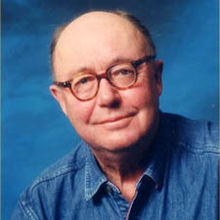
\includegraphics[width=2.5cm]{img/needham.jpg}
  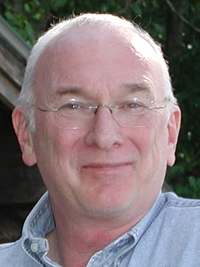
\includegraphics[width=2.5cm]{img/schroeder.jpg}}
   \end{column}
    \end{columns}

}

\frame{
    \frametitle{Introduction}
    \framesubtitle{Historical facts}
           \begin{columns}
    \begin{column}{4cm}
 \visible<4>{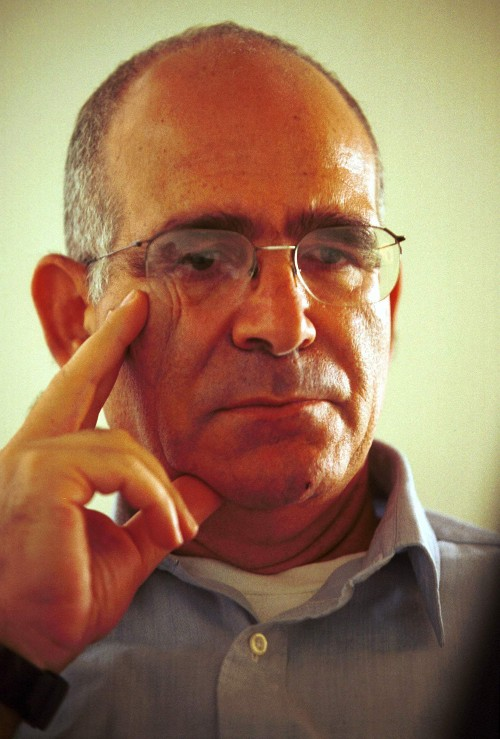
\includegraphics[width=2cm]{img/dolev.jpg}
  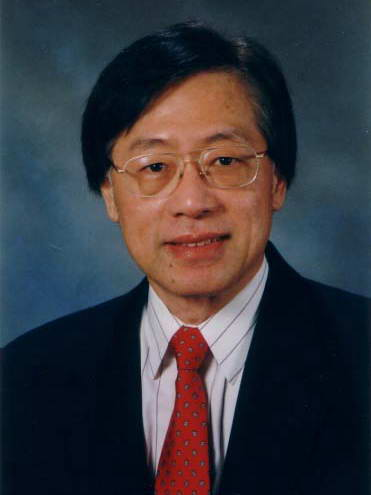
\includegraphics[width=2cm]{img/yao.jpg}}
             \end{column}
  \begin{column}{7cm}
  \begin{itemize}
        \item Dolev and Yao further developed the attacker model; \pause
        \begin{itemize}
      	    \item \textbf{\textit{The attacker has complete control of the communication channels (respecting cryptography)}};\pause
        \end{itemize}
        \item Nowadays, the Dolev-Yao threat model is the most widely accepted model to analyse security protocols; \pause        
    \end{itemize}
   \end{column}
    \end{columns}

       
}

\frame{
    \frametitle{Human-centered computing}
    \framesubtitle{Definitions}
    \begin{center}
\includegraphics[height=2cm,width=8cm]{img/human-touch.jpg}\end{center}
    \begin{itemize}
        \item Concerned with computing as it relate to human condition; \pause
        \item Research in human-centred computing has multiple goals; \pause
        \item  Focus on the ways that human beings adopt, adapt, and organise their lives around computational technologies; \pause
        \item This inherently brings a social aspect to computing!      
        \end{itemize}
  }

  
\frame{
    \frametitle{Introduction}
    \framesubtitle{Motivation for Human Centric Protocol Security}
          \begin{columns}
    \begin{column}{6cm}
    \begin{itemize}
        \item<1-> When put in practice, protocols' assumptions that involves human-device and human-human interaction have to be implemented;        
        \item<2-> They are then replaced by dynamic user-interactions 
            \end{itemize}
               \end{column}
    \begin{column}{5cm}
  \visible<1->{
\includegraphics[width=5cm]{img/interaction.jpg}}
   \end{column}
    \end{columns}

  }
  
  
\frame{
    \frametitle{Introduction}
    \framesubtitle{Motivation for Human Centric Protocol Security}
    \begin{itemize}
        \item Even protocols verified under Dolev-Yao threat model assumptions might be susceptible to attacks when implemented due to some reasons, which may include:\pause      
        \begin{itemize}            
            \item Clear usability problems – the user must have unrealistic capabilities to perform his activities;\pause            
            \item The assumptions are too big/strong or too generic – it is often necessary to assume that previous steps were successfully performed, or that the user is capable of performing some kind of operation.
        \end{itemize}
    \end{itemize}
  }

\frame{
    \frametitle{Introduction}
    \framesubtitle{How do we sort this out?}
    \begin{center}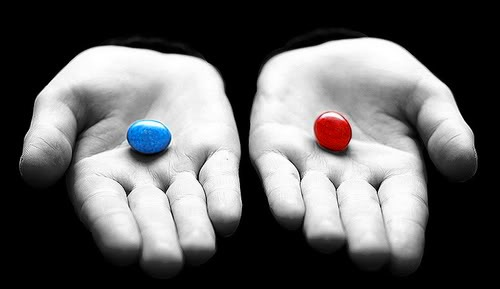
\includegraphics[width=7cm]{img/choice.jpg}\end{center}
    \begin{itemize}
        \item Clearly we have at least two choices: \pause
        \begin{itemize}            
            \item We change the user interaction;\pause
            \item We change the assumption.
        \end{itemize}
    \end{itemize}
  }

\frame{
    \frametitle{Introduction}
    \framesubtitle{Why changing the user is not a good idea?}
              \begin{columns}
    \begin{column}{4cm}
     
\includegraphics[width=4cm]{img/good_user.jpg}
             \end{column}
  \begin{column}{7cm}
    \begin{itemize}
        \item User interaction is per se unpredictable;\pause
        \item Modelling the user is very hard;\pause
        \item Constructing a tool for that is complicated;\pause
        \item The user is not part of the problem, but part of the solution!
    \end{itemize}
       \end{column}
    \end{columns}
  }

\frame{
	\frametitle{Introduction}
	\framesubtitle{Motivation}
    \begin{itemize}    
    \item Dolev-Yao threat model represents the most powerful attacker possible;\pause
    
    \item However, this powerful attacker is not realistic in certain scenarios;\pause
    
    \item Workarounds to protect agains unrealistic attacks may introduce security problems;\pause
    
    \item Despite the fact that the security flaws are introduced during the implementation of the procotol, its cause is often an inaccurate assumption which may have been forced by an unrealistic threat model
    \end{itemize}
  }

%=============%
% New Section %
%=============%
\section{Ceremonies}

\frame{
    \frametitle{Security Ceremonies}
    Ellison introduced the concept of a broader view to security protocols called ``ceremony'' \pause
    \begin{figure}[htbp]        
    \centering
    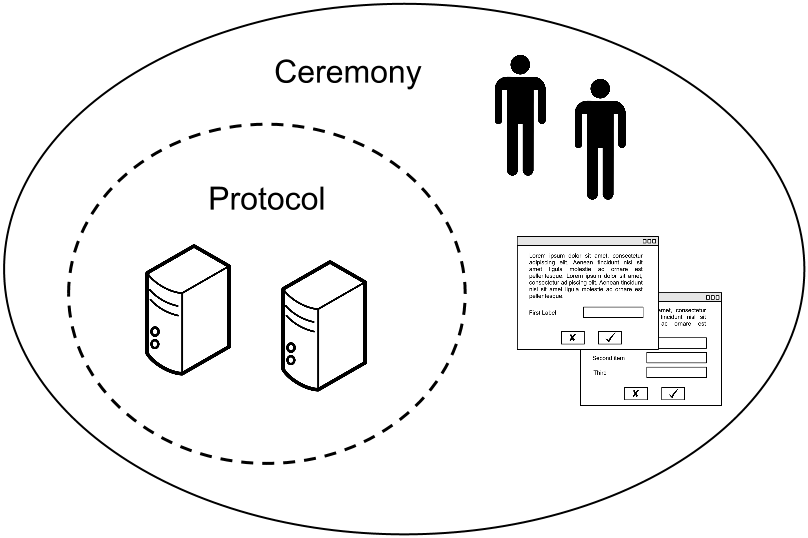
\includegraphics[width=.7\textwidth]{img/ceremony-protocol.png}
    \label{fig:ceremony-protocol}
\end{figure}
}

\frame{
	\frametitle{Ceremonies}
   \begin{itemize}
   \item Security protocols are sequence of interactions among entities designed to achieve a certain end;\pause
   
   \begin{itemize}
       \item Goals are (not limited to):\pause
       \begin{itemize}
           \item Authentication, Key distribution, Secrecy, Anonymity, etc\pause
       \end{itemize}
   \end{itemize}
   
   \item Ceremonies include in addition to protocols:\pause
   
   \begin{itemize}
       \item new node types (humans, user interfaces, etc);\pause
       
       \item new communication channels (human-device, human-human);\pause
       
       \item additional operations which were previously out-of-bounds (user interaction, pre-key distribution).\pause
   \end{itemize}
   \item In a protocol specification, we define assumptions to represent out-of-bound operations;\pause
   
   \item In ceremonies we break down these assumptions into smaller and well described assumptions.
   
   \end{itemize}
 }

\frame{
	\frametitle{Security Ceremonies}
	          \begin{columns}
    \begin{column}{6cm}
    \begin{itemize}
    \item<+-> A ceremony allows more detailed analysis of a protocol
    \item<+-> Assumptions are more precise and well described
    \item<+-> A Dolev-Yao attacker for ceremonies is not always consistent with real world threats
       \begin{itemize}
     	\item An attacker capable of modifying (or replaying) a ``speech'' packet in a human-human medium is unrealistic if this communication happens in person
   \end{itemize}
   
    %\item<+-> The description attacker capabilities for ceremonies scope requires finer granularity in its description       
    \end{itemize}
    \end{column}
    \begin{column}{5cm}
   \visible<1->{
\includegraphics[width=5cm]{img/brain.jpg}}
   \end{column}
    \end{columns}
  }
  
  

\frame{
	\frametitle{Ceremony Verification}
	\framesubtitle{Justification}
   \begin{itemize}
   \item A more human-centric security view;\pause
   
   \item Designing more realistic ceremonies;\pause
   
   \item Assist the human peer to assess the threat level he is subject to;\pause
   
   \item By not overstating assumptions we inherently make them plausible and achievable.
   \end{itemize}
 }



\frame{
	\frametitle{Security Ceremonies}
	    \begin{center}
\includegraphics[width=5cm]{img/attacker.jpg}\end{center}
    \begin{itemize}
    \item If a ceremony is secure against a Dolev-Yao attacker, the same ceremony will be secure against a weaker attacker; \pause
    \item However, to guarantee that a ceremony is secure against a such powerful attacker, we have to include very complex mechanisms.
        \end{itemize}
  }
  
\frame{
	\frametitle{Security Ceremonies}
    \begin{itemize}
    \item<+-> By doing that, a new threat is introduced, which is the fact that the user is likely to try to circumvent the security mechanisms in order to accomplish his/her tasks; 
    \item<+-> A more realistic threat model can prevent the user from being overloaded, and consequently make the ceremony more usable and secure
    \end{itemize}
      \visible<1->{\begin{center}
\includegraphics[width=5cm]{img/overload.jpg}\end{center}}
  }

\section{Premises for  Threat Modelling}

\frame{
	\frametitle{Premises for Ceremonies Threat Modelling}
		          \begin{columns}
    \begin{column}{7cm}
    \begin{itemize}
    \item<+-> No being is omnipotent in human-human channels;
    \item<+-> Omnipotency in the human-device channel is not always realistic;
    \item<+-> A threat model including human peers should be constrained by the laws of physics;
    \item<+-> Humans are capable of performing basic information recall or mathematical operations;
    \item<+-> One should never use more crypto than needed.
    \end{itemize}
           \end{column}
    \begin{column}{4cm}
  \visible<1->{
\includegraphics[width=4cm]{img/devil.jpg}}
   \end{column}
    \end{columns}
  }  
  
\section{Proposed Threat Model}

%\frame{
%	\frametitle{Proposed Threat Model}
%	\framesubtitle{Justification}
%    \begin{itemize}
%    \item Reasons for ceremony security flaws are not necessarely related to the network channel.
%    \item Therefore we can find secure protocols that are not secure when implemented
%    \item We cannot assure that the expected security properties assumed in the protocol design will hold in the ceremony.    
%    \end{itemize}
%  } 

\frame{
	\frametitle{The Ever Changing Threat Model}
	\framesubtitle{Scenario}
    \begin{itemize}
    \item We introduce two new possible communication channels.\pause
    \end{itemize}
   \begin{figure}[htbp]
   \centering
   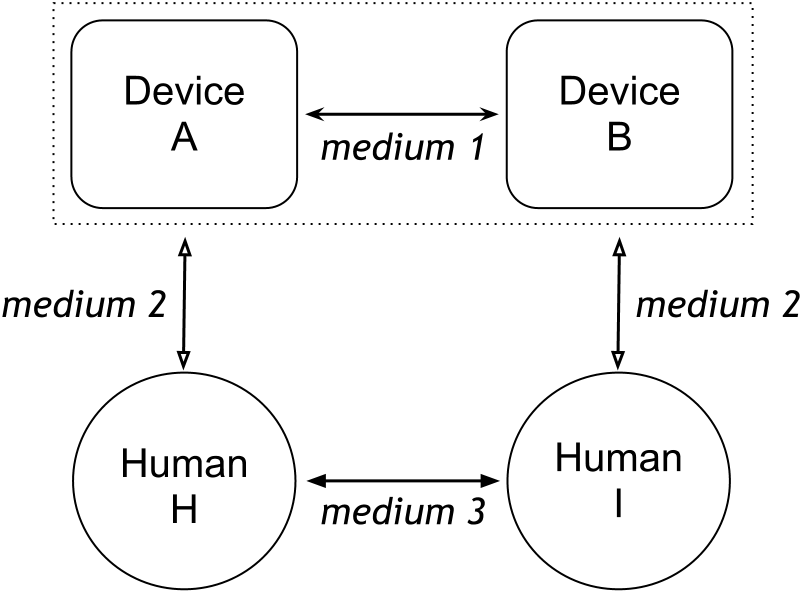
\includegraphics[width=.6\textwidth]{img/ceremony-mediums.png}
   %\caption{Ceremony communication mediums}
   \label{fig:channels}
   \end{figure}
} 

\frame{
	\frametitle{Proposed Threat Model}
	\framesubtitle{We also consider...}
	 \begin{center}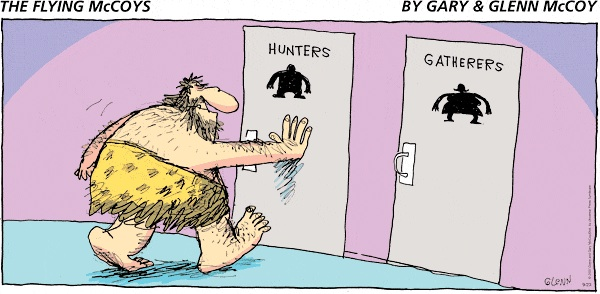
\includegraphics[width=5cm]{img/hunters.jpg}\end{center}
    \begin{itemize}
    \item Humans make decisions regarding their security based on the evaluation of the threat level they are subject to: \pause
        \begin{itemize}
    	\item Humans had to decide whether to engage into attacks to become hunters or keep a way of life of gatherers;\pause
	\item Inherent faculty of human nature;\pause
	\item Some attacks may be thwarted, but inherently this will attract the human nature.
    \end{itemize}
    \end{itemize}
  }  
  
\frame{
	\frametitle{Human Centred Threat Model}
				          \begin{columns}
    \begin{column}{7cm}
    \begin{itemize}
    \item<+-> Considering worst case is not always the best option since it degrades usability;
    \item<+-> The threat model must be adaptive;
    \item<+-> For network communication (device-device channel) we will usually assume a Dolev-Yao attacker;
    \item<+-> A threat model for ceremonies must be ceremony-dependent and context-dependent.
%    \item The existence of a standardised  threat model scenario is paramount to the establishment of security goals of ceremonies.
    \end{itemize}
                               \end{column}
    \begin{column}{4cm}
  \visible<1->{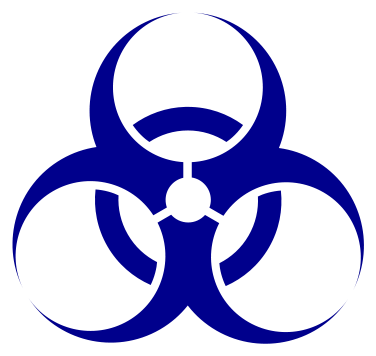
\includegraphics[width=4cm]{img/threat.png}}
   \end{column}
    \end{columns}
  }  
  
\frame{
	\frametitle{Proposed Threat Model}
	\framesubtitle{How can we do it?}
    \begin{itemize}
    \item We start from Dolev-Yao, and then we remove one or more capabilities from the attacker;\pause
    \item Our final goal is to measure the security of ceremonies against a Dolev-Yao attacker with a smaller set of capabilities;\pause
    \item This approach will also help us to reuse some of the abstract verification techniques and tools already in use for security protocols;\pause
    \item Verify that ceremonies are secure against a realistic attacker.
    \end{itemize}

}    
\frame{
	\frametitle{Proposed Threat Model}
	\framesubtitle{Notation}
   \begin{itemize}
   	\item ``DY'' is a Dolev-Yao attacker
	
	\item ``DY-BR'' means a Dolev-Yao attacker without the blocking and replaying capabilities. 
	
	\item All the logical connectives have their usual meaning.
	
	\item The set knows(X), represents the set of knowledge of an agent X in the protocol.
   \end{itemize}
}    

\frame{
	\frametitle{Proposed Threat Model}
	\framesubtitle{Capabilities}
    \begin{columns}
    \begin{column}{6cm}
     \begin{itemize}
         \item<+-> Eavesdrop
         \item<+-> Initiate
         \item<+-> Atomic Break Down
         \item<+-> Crypto
         \item<+-> Block
         \item<+-> Fabricate
         \item<+-> Spoof
         \item<+-> re-Order
    \end{itemize}
    \visible<+->{\textit{Some of the characteristics are achieved by the combination of our definitions (e.g. Replaying = Eavesdrop + Initiate)}}
                \end{column}
  \begin{column}{5cm}
  \visible<1->{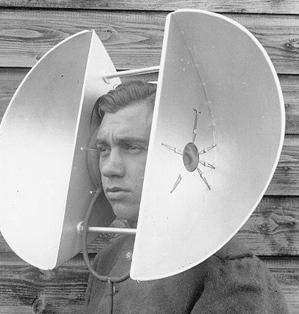
\includegraphics[width=5cm]{img/eavesdrop.jpg}}
   \end{column}
    \end{columns}
}  

\frame{
	\frametitle{Proposed Threat Model}
	\framesubtitle{Capabilities}
   \begin{itemize}

	
	\item Examples:
	 \begin{itemize}
   	\item Modifying (M) messages on the communication channels can be defined as the use of \textbf{Block $+$ Initiate}
	\item Replaying (R) messages can be represented as \textbf{Eavesdrop $+$ Initiate} or \textbf{Eavesdrop $+$ Spoof} 
	\end{itemize}

	
   \end{itemize}
}    

\frame{
	\frametitle{Proposed Threat Model}
	\framesubtitle{Secondary Notation}
   \begin{itemize}
   	\item We start with no threat model.
	
	\item The attacker has ``no capabilities'' (N).
	
	\item We add to the (N) attacker the desired capabilities.
	
	\item Examples:
	
	 \begin{itemize}
   	\item N + E for eavesdrop only,
	\item N + EB for eavesdrop and block only.
	\end{itemize}
	
	\item DY-IDBRSM = N+E

	
   \end{itemize}
}    

\section{Example scenario: Bluetooth}

\frame{
	\frametitle{Example scenario: Bluetooth Pairing Protocol}
	\framesubtitle{Overview}
	    \begin{columns}
   \begin{column}{8cm}
   \begin{itemize}
		\item Protocol designed to allow one device to recognise and connect to another. 
		
       \item Our focus is on the \textbf{Secure Simple Pairing (SSP)} (bluetooth 2.1 onwards) using the \textbf{Numeric Comparison} mode:
       
       \begin{itemize}		
			\item designed for devices capable of displaying digits (a six digit number) and accepting user inputs (``yes'' or ``no'') 
			
			\item The device displays six digit numbers on both devices. 
			
			\item If the digits are equal, the pairing is successful
		\end{itemize}
   \end{itemize}\   \end{column}
 \begin{column}{3cm}
 
\includegraphics[width=3cm]{img/bluetoothman.jpg}
  \end{column}
   \end{columns}
}   

\frame{
	\frametitle{Example scenario: Bluetooth Pairing Protocol}
	\framesubtitle{Legacy Pairing}
   \begin{itemize}
		\item Pairing is performed in a way where both devices are required to enter a common PIN to establish the connection
		
		\item Three input types:
		
		\begin{itemize}
			\item Fixed PIN number is used (e.g. 1234) % For devices with limited input capabilities
			
			\item Numeric input % devices with numeric keyboard only
			
			\item Alpha-numeric input % (e.g. modern mobile phones and computers).
		\end{itemize}				
   \end{itemize}
}   
	
\frame{
	\frametitle{Example scenario: Bluetooth Pairing Protocol}
	\framesubtitle{Secure Simple Pairing (SSP)}
   \begin{itemize}
		\item Solves several flaws that allowed attackers to deploy man-in-the-middle (MITM) attacks on earlier versions
		
		\item Defines four different association modes
		
		\item Simplifies the pairing process from the user's point of view     \end{itemize}
}   

\frame{
	\frametitle{Example scenario: Bluetooth Pairing Protocol}
	\framesubtitle{Secure Simple Pairing (SSP)}
   \begin{itemize}
		\item SSP association modes:
		
		\begin{itemize}
			\item {\textbf{Numeric Comparison}}
			
			\item Just Works
			
			\item Out of band (OOB)
			
			\item Passkey entry
		\end{itemize}
   \end{itemize}
}   

\frame{
	\frametitle{Example scenario: Bluetooth Pairing Protocol}
	\framesubtitle{Secure Simple Pairing (SSP)}
   \begin{itemize}
   		\item Numeric Comparison mode
   		
	    		\begin{itemize}		
			\item designed for devices capable of displaying digits (a six digit number) and accepting user inputs (``yes'' or ``no''). 
			
			\item The device displays six digit numbers on both devices and the users are asked whether the numbers are the equal on both devices. 
			
			\item If the digits are equal, the pairing is successful
			\end{itemize}
	\end{itemize}
}

\frame{
	\frametitle{Example scenario: Bluetooth Pairing Protocol}
	\framesubtitle{Attacks}
   \begin{itemize}
		\item The association modes are designed under assumptions that imply in a weaker threat model for the pairing protocol.		
		\item Legacy mode
		
		\begin{itemize}
			\item Device-device medium (DD) is designed considering a DY attacker
			
			\item Human-device (HD) and human-human mediums (HH) are assumed to have no attackers.
			
			\item A ceremony analysis can easily find an attack if we add the capability of eavesdropping to the attacker on either HD or HH mediums. 
			
			\item The attacker learns the PIN by eavesdropping those mediums (hearing the PIN value) and with that, he can decode all the messages. %This works similarly to the attack described in \cite{shaked:2005}, but without the need of deploying a brute force attack on the PIN. This attack would easily be captured when verifying this protocol as a ceremony.
		\end{itemize}
	\end{itemize}
}


\frame{
	\frametitle{Example scenario: Bluetooth Pairing Protocol}
	\framesubtitle{Attacks}
   \begin{itemize}
		\item The association modes are designed under assumptions that imply in a weaker threat model for the pairing protocol. 
		
		\item SSP
		
		\begin{itemize}
			\item Each association mode also needs to be analysed under a different threat model
			
			\item We will focus on the numeric comparison mode
		\end{itemize}
	\end{itemize}
}

\frame{
	\frametitle{Example scenario: Bluetooth Pairing Protocol}
	\framesubtitle{Secure Simple Pairing (SSP) -- Numeric Comparison}
\begin{figure}[h!]
\centering
\begin{tabular}{c c c c c c }
M1. & $B$   & $\xrightarrow[DD]{}$ & $A$   & : & $C_b = f1(pk_B, pk_A, N_b, 0)$ \\
M2. & $A$   & $\xrightarrow[DD]{}$ & $B$   & : & $N_a$ \\
M3. & $B$   & $\xrightarrow[DD]{}$ & $A$   & : & $N_b$ \\
M4. & $A$   & $\xrightarrow[HD]{}$ & $U_A$ & : & $V_a = g(pk_A, pk_B, N_a, N_b)$ \\
M5. & $B$   & $\xrightarrow[HD]{}$ & $U_B$ & : & $V_b = g(pk_A, pk_B, N_a, N_b)$ \\
M6. & $U_A$ & $\xrightarrow[HH]{}$ & $U_B$ & : & $V_a$ \\
M7. & $U_B$ & $\xrightarrow[HH]{}$ & $U_A$ & : & $V_b$ \\
\end{tabular}
\end{figure}
}


\frame{
	\frametitle{Example scenario: Bluetooth Pairing Protocol}
	\framesubtitle{Secure Simple Pairing (SSP) -- Numeric Comparison}
	
   \begin{figure}[htbp]        
   \centering
   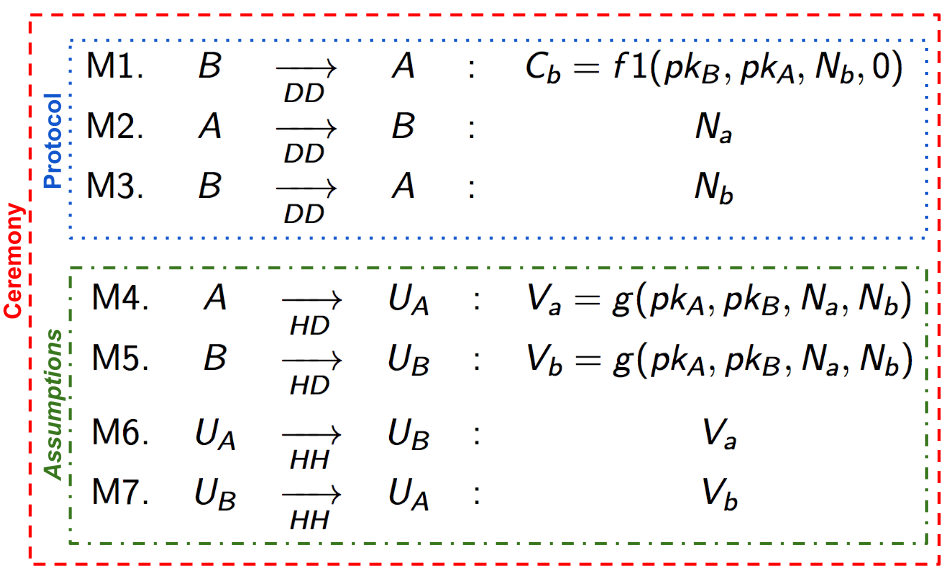
\includegraphics[width=.95\textwidth]{img/bluetooth-ceremony.png}
   \label{fig:ceremony-protocol}
   \end{figure}

}

\frame{
	\frametitle{Example scenario: Bluetooth Pairing Protocol}
	\framesubtitle{Secure Simple Pairing (SSP) -- Analysis}
	\begin{theorem}[Numeric Comparison + DY] \label{thr:dy} If the protocol messages $M_1$ to $M_7$ are run against a DY attacker, the attacker can prevent $U_A$ from learning $V_a$ or $V_b$ and $U_B$ from learning $V_b$ or $V_a$, forcing them to learn $V_i$ instead.
 \begin{displaymath}
   \begin{split}
	 \frac{M_{1...7} \cup DY}
{\begin{split}
V_a \land V_b \land V_i \in knows(I) \land \\
V_a \notin knows(A) \land V_b \notin knows(A) \land \\
V_b \notin knows(B) \land V_a \notin knows(B) \land \\
V_i \in knows(U_A) \land V_i \in knows(U_B)  \end{split}}
   \end{split}
 \end{displaymath}

\end{theorem}
}

\frame{
	\frametitle{Example scenario: Bluetooth Pairing Protocol}
	\framesubtitle{Secure Simple Pairing (SSP) -- Analysis -- NC + DY}
   \begin{itemize}
		\item Assuming the attacker $I$ initiated two parallel pairing sessions with $A$ and $B$ during Messages $M_1$ to $M_3$:
	\end{itemize}
\begin{figure}[h!]
\centering
\begin{tabular}{c c c c c c }
M4. & $A$   & $\xrightarrow[HD]{}$ & $U_A$ & : & $V_a' = g(pk_A, pk_I, N_a, N_i)$ {\color{red}(Blocked)}\\
M5. & $B$   & $\xrightarrow[HD]{}$ & $U_B$ & : & $V_b' = g(pk_I, pk_B, N_i, N_b)$ {\color{red}(Blocked)}\\
M4'. & $I$   & $\xrightarrow[HD]{}$ & $U_A$ & : & $V_i$ {\color{red}(Chosen by the attacker)}\\
M5'. & $I$   & $\xrightarrow[HD]{}$ & $U_B$ & : & $V_i$ {\color{red}(Chosen by the attacker)}\\
M6. & $U_A$ & $\xrightarrow[HH]{}$ & $U_B$ & : & $V_i$ \\
M7. & $U_B$ & $\xrightarrow[HH]{}$ & $U_A$ & : & $V_i$ \\
\end{tabular}
\end{figure}	
}

\frame{
	\frametitle{Example scenario: Bluetooth Pairing Protocol}
	\framesubtitle{Secure Simple Pairing (SSP) -- Analysis}
   \begin{itemize}
		\item Although first attack described is plausible in real world scenarios, it is very difficult to be deployed
		
		\item An attacker would have to corrupt both devices as well as start parallel sessions with both users during a short period of time
		
		\item By removing capabilities ``Block'' and ``Initiate'' from the attacker, we can analyse the protocol further, and possibly find other (more) relevant attacks
	\end{itemize}
}

\frame{
	\frametitle{Example scenario: Bluetooth Pairing Protocol}
	\framesubtitle{Secure Simple Pairing (SSP) -- Analysis}
\begin{theorem}[Numeric Comparison + Ad. Threat Model V1] \label{thr:atm:v1} If the protocol messages $M_1$ to $M_3$ are run against a DY attacker; the messages $M_4$ to $M_5$ are run against a N+E attacker; and messages $M_6$ to $M_7$ are run against a DY attacker, the attacker can prevent $U_A$ from learning $V_b$ and $U_B$ from learning $V_a$, forcing them to learn the repetition (replay) of $V_a$ and $V_b$ (respectively) instead.
\[
\frac{(M_{1...3} \cup DY) \land (M_{4...5} \cup N+E) \land ) (M_{6...7} \cup DY)}
{V_a \land V_b \in knows(I) \land V_a \notin knows(B) \land V_b \notin knows(A) }
\]
\end{theorem}
}


\frame{
	\frametitle{Example scenario: Bluetooth Pairing Protocol}
	\framesubtitle{Secure Simple Pairing (SSP) -- Analysis}
   \begin{itemize}
		\item Assuming the attacker $I$ initiated two parallel pairing sessions with $A$ and $B$ during Messages $M_1$ to $M_3$:
	\end{itemize}
\begin{figure}[h!]
\centering
\begin{tabular}{c c c c c c }
M4. & $A$   & $\xrightarrow[HD]{}$ & $U_A$ & : & $V_a' = g(pk_A, pk_I, N_a, N_i)$ \\
M5. & $B$   & $\xrightarrow[HD]{}$ & $U_B$ & : & $V_b' = g(pk_I, pk_B, N_i, N_b)$ \\
M6. & $U_A$ & $\xrightarrow[HH]{}$ & $U_B$ & : & $V_a'$ {\color{red}(Blocked)}\\
M7. & $U_B$ & $\xrightarrow[HH]{}$ & $U_A$ & : & $V_b'$ {\color{red}(Blocked)}\\
M6'. & $I$ & $\xrightarrow[HH]{}$ & $U_B$ & : & $V_b'$ {\color{red}($V_b'  \in knows(I)$ by M5 or M7)} \\
M7'. & $I$ & $\xrightarrow[HH]{}$ & $U_A$ & : & $V_a'$ {\color{red}($V_b' \in knows(I)$ by M4 or M6)} \\
\end{tabular}
\end{figure}	
}

\frame{
	\frametitle{Example scenario: Bluetooth Pairing Protocol}
	\framesubtitle{Secure Simple Pairing (SSP) -- Analysis}
   \begin{itemize}
		\item This second attack is completely unrealistic 
		
		\item The attacker would have to block a communication between two humans and then replay some data over a channel where the user would easily notice if some other party wanted to spoof the identity of the sender % -- depende do Spoof do comentario de antes ...}. 
		
		\item In this case, the attack does not exist in practice
	\end{itemize}
}

\frame{
	\frametitle{Example scenario: Bluetooth Pairing Protocol}
	\framesubtitle{Secure Simple Pairing (SSP) -- Analysis}
\begin{theorem}[NumComp + Ad. Threat Model V2] \label{thr:atm:v2} If the protocol messages $M_1$ to $M_3$ are run against a DY attacker and the messages $M_4$ to $M_7$ are run against a N+E attacker the attacker cannot produce any relevant attack.
\[
\frac{(M_{1...3} \cup DY) \land (M_{4...7} \cup N+E) }
{\emptyset}
\]
\end{theorem}
}

\frame{
	\frametitle{Example scenario: Bluetooth Pairing Protocol}
	\framesubtitle{Secure Simple Pairing (SSP) -- Analysis}
   \begin{itemize}
		\item Assuming the attacker $I$ initiated two parallel pairing sessions with $A$ and $B$ during Messages $M_1$ to $M_3$:
	\end{itemize}
\begin{figure}[h!]
\centering
\begin{tabular}{c c c c c c }
M4. & $A$   & $\xrightarrow[HD]{}$ & $U_A$ & : & $V_a' = g(pk_A, pk_I, N_a, N_i)$ \\
M5. & $B$   & $\xrightarrow[HD]{}$ & $U_B$ & : & $V_b' = g(pk_I, pk_B, N_i, N_b)$ \\
M6. & $U_A$ & $\xrightarrow[HH]{}$ & $U_B$ & : & $V_a'$ \\
M7. & $U_B$ & $\xrightarrow[HH]{}$ & $U_A$ & : & $V_b'$ \\
\end{tabular}
\end{figure}
	
\begin{block}{The attack fails}
	Since $V_a' \neq V_b'$ and the attacker cannot initiate communication using the $HD$ and $HH$ channels, there is no realistic attack on the protocol.
\end{block}
}

\section{Gains Under a Realistic Threat Model}
\frame{
	\frametitle{Gains Under a Realistic Threat Model}


   \begin{itemize}
		\item The misunderstanding of the correct threat model would lead to us to the incorrect conclusion that it is not secure
		
		\item The ceremony for the bluetooth association protocol can be described avoiding these conclusions
		
		\item The ceremony could enforce the use of a correct threat model choice at implementation level
		
		%\item Example: an application could dynamically allow/block different association modes depending on the environment
				
		\item This kind of ceremony potentially trains users to detect different threat models
	\end{itemize}
	}

\frame{
	\frametitle{Where to go now?}
	%\framesubtitle{}
			    \begin{columns}
   \begin{column}{3cm}
	  
\includegraphics[width=3cm]{img/wheretogo.jpg}
  
 \end{column}
 \begin{column}{7cm}
\begin{itemize}
		\item Specification of the threat model using an abstract verification method
		
		\item Automation for testing and design of security ceremonies
		
		\item Refining model to cope with more channels
		
		\item Redefining new ceremonies for old problems.
	\end{itemize}
  \end{column}
   \end{columns}

}


\frame{
	\frametitle{Gains Under a Realistic Threat Model}
	\framesubtitle{Gains in Bluetooth Pairing Ceremonies}
   \begin{itemize}
		\item Pairing under the JW mode:
		
		\begin{itemize}
		\item The application should scan the area and check whether there are more bluetooth enabled devices around.
		\item If more than one is found, the JW mode should not be available.
		\item If only one device is found, the JW mode can be securely used.
		\end{itemize}
	\end{itemize}
}


\section{Final Remarks}

\frame{
	\frametitle{Concluding Remarks}
%	\framesubtitle{Conclusions}
    \begin{itemize}
		\item The use of a worst-case scenario threat model is justifiable in security protocol scenarios;\pause
		\item However, the same cannot be said for  a human centric approach;\pause
		\item  Human agents executing security ceremonies are constrained by the laws of physics and usual capabilities expected from human beings;\pause
		\item The existence of a extremely powerful agent is not plausible in some real-world scenarios.
	\end{itemize}
}

%\frame{
%	\frametitle{Concluding Remarks}
%%	\framesubtitle{Conclusions}
%    \begin{itemize}
%		\item Our approach is based on a well established model for security protocols
%		
%		\item We weaken the attacker to match the premises for human-device interaction and human-human interaction
%		
%		\item Our model helps security protocols and ceremony designers to develop ceremonies:
%			
%		\begin{itemize}
%		\item using reasonable assumptions
%		
%		\item tailored to the real capabilities of the attacker
%				
%		\item that do not contain unnecessary protection mechanisms to unrealistic attacks
%        	\end{itemize}	
%	\end{itemize}
%}

\frame{
	\frametitle{Discussion}
\begin{itemize}
\item How do you relate the ideas of ceremonies to threat models?\pause
\item Is it reasonable to use this threat model for security protocols?\pause
\item Can you describe a situation where you could gain leverage by using this threat model?
\end{itemize}
}

{
\usebackgroundtemplate{
\includegraphics[width=\paperwidth,
height=\paperheight]{../reusable_images/fundo_capa.png}}
\begin{frame}

{\LARGE Questions????}

\end{frame}
}

{
\usebackgroundtemplate{
\includegraphics[width=\paperwidth,
height=\paperheight]{../reusable_images/fundo_capa.png}}
\begin{frame}

\includegraphics[scale=0.8]{../reusable_images/cc_logo_arge.png}\hspace{0.5cm} 

\includegraphics[scale=0.95]{../reusable_images/by.png}

\vspace{1cm}
This work is licensed under the Creative Commons Attribution 4.0 International License. To view a copy of this license, visit http://creativecommons.org/licenses/by/4.0/.
\end{frame}
}

\end{document}
